% Created by tikzDevice version 0.12.6 on 2024-03-21 19:37:41
% !TEX encoding = UTF-8 Unicode
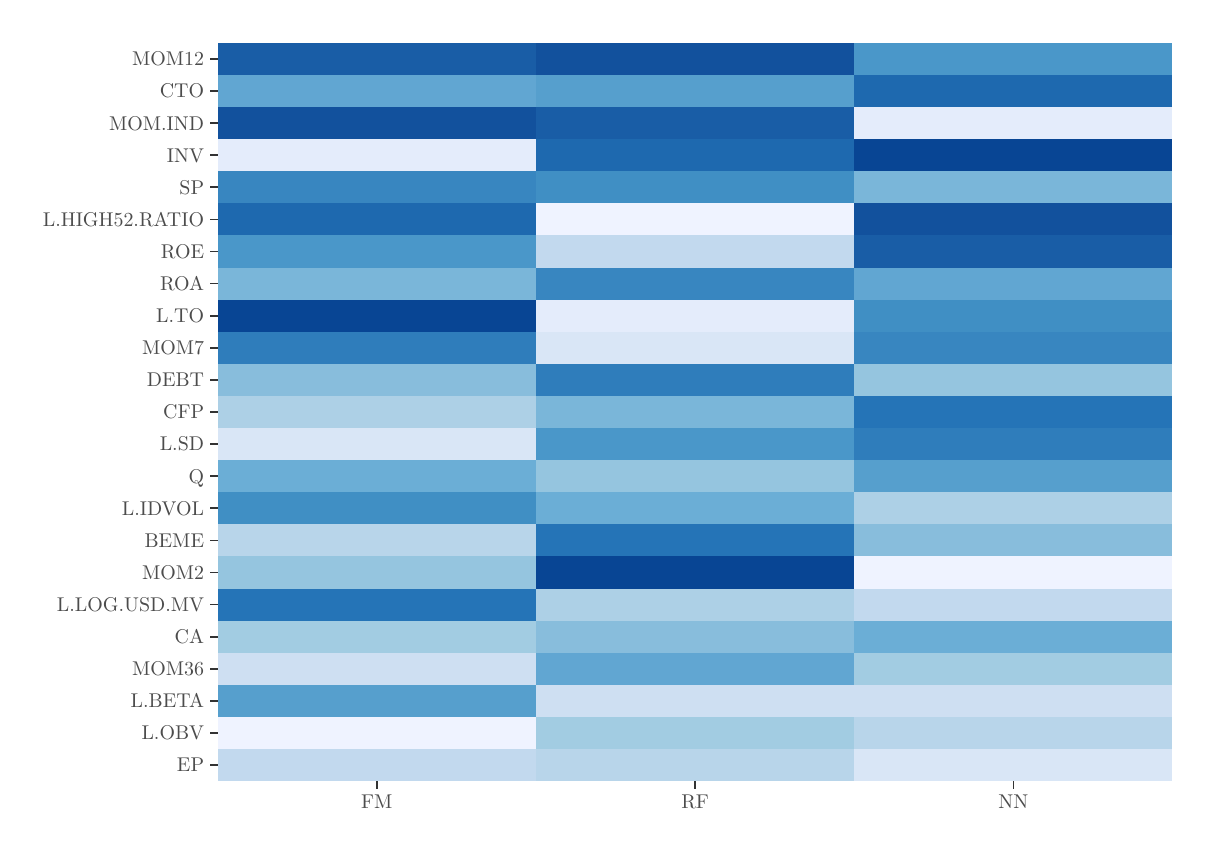
\begin{tikzpicture}[x=1pt,y=1pt]
\definecolor{fillColor}{RGB}{255,255,255}
\path[use as bounding box,fill=fillColor,fill opacity=0.00] (0,0) rectangle (419.17,289.08);
\begin{scope}
\path[clip] (  0.00,  0.00) rectangle (419.17,289.08);
\definecolor{drawColor}{RGB}{255,255,255}
\definecolor{fillColor}{RGB}{255,255,255}

\path[draw=drawColor,line width= 0.6pt,line join=round,line cap=round,fill=fillColor] (  0.00,  0.00) rectangle (419.17,289.08);
\end{scope}
\begin{scope}
\path[clip] ( 68.69, 16.81) rectangle (413.67,283.58);
\definecolor{fillColor}{gray}{0.92}

\path[fill=fillColor] ( 68.69, 16.81) rectangle (413.67,283.58);
\definecolor{drawColor}{RGB}{255,255,255}

\path[draw=drawColor,line width= 0.6pt,line join=round] ( 68.69, 22.61) --
	(413.67, 22.61);

\path[draw=drawColor,line width= 0.6pt,line join=round] ( 68.69, 34.21) --
	(413.67, 34.21);

\path[draw=drawColor,line width= 0.6pt,line join=round] ( 68.69, 45.81) --
	(413.67, 45.81);

\path[draw=drawColor,line width= 0.6pt,line join=round] ( 68.69, 57.40) --
	(413.67, 57.40);

\path[draw=drawColor,line width= 0.6pt,line join=round] ( 68.69, 69.00) --
	(413.67, 69.00);

\path[draw=drawColor,line width= 0.6pt,line join=round] ( 68.69, 80.60) --
	(413.67, 80.60);

\path[draw=drawColor,line width= 0.6pt,line join=round] ( 68.69, 92.20) --
	(413.67, 92.20);

\path[draw=drawColor,line width= 0.6pt,line join=round] ( 68.69,103.80) --
	(413.67,103.80);

\path[draw=drawColor,line width= 0.6pt,line join=round] ( 68.69,115.40) --
	(413.67,115.40);

\path[draw=drawColor,line width= 0.6pt,line join=round] ( 68.69,127.00) --
	(413.67,127.00);

\path[draw=drawColor,line width= 0.6pt,line join=round] ( 68.69,138.60) --
	(413.67,138.60);

\path[draw=drawColor,line width= 0.6pt,line join=round] ( 68.69,150.19) --
	(413.67,150.19);

\path[draw=drawColor,line width= 0.6pt,line join=round] ( 68.69,161.79) --
	(413.67,161.79);

\path[draw=drawColor,line width= 0.6pt,line join=round] ( 68.69,173.39) --
	(413.67,173.39);

\path[draw=drawColor,line width= 0.6pt,line join=round] ( 68.69,184.99) --
	(413.67,184.99);

\path[draw=drawColor,line width= 0.6pt,line join=round] ( 68.69,196.59) --
	(413.67,196.59);

\path[draw=drawColor,line width= 0.6pt,line join=round] ( 68.69,208.19) --
	(413.67,208.19);

\path[draw=drawColor,line width= 0.6pt,line join=round] ( 68.69,219.79) --
	(413.67,219.79);

\path[draw=drawColor,line width= 0.6pt,line join=round] ( 68.69,231.39) --
	(413.67,231.39);

\path[draw=drawColor,line width= 0.6pt,line join=round] ( 68.69,242.98) --
	(413.67,242.98);

\path[draw=drawColor,line width= 0.6pt,line join=round] ( 68.69,254.58) --
	(413.67,254.58);

\path[draw=drawColor,line width= 0.6pt,line join=round] ( 68.69,266.18) --
	(413.67,266.18);

\path[draw=drawColor,line width= 0.6pt,line join=round] ( 68.69,277.78) --
	(413.67,277.78);

\path[draw=drawColor,line width= 0.6pt,line join=round] (126.18, 16.81) --
	(126.18,283.58);

\path[draw=drawColor,line width= 0.6pt,line join=round] (241.18, 16.81) --
	(241.18,283.58);

\path[draw=drawColor,line width= 0.6pt,line join=round] (356.17, 16.81) --
	(356.17,283.58);
\definecolor{fillColor}{RGB}{37,116,183}

\path[fill=fillColor] (183.68, 98.00) rectangle (298.67,109.60);
\definecolor{fillColor}{RGB}{136,189,220}

\path[fill=fillColor] (183.68, 63.20) rectangle (298.67, 74.80);
\definecolor{fillColor}{RGB}{122,182,217}

\path[fill=fillColor] (183.68,144.39) rectangle (298.67,155.99);
\definecolor{fillColor}{RGB}{86,159,205}

\path[fill=fillColor] (183.68,260.38) rectangle (298.67,271.98);
\definecolor{fillColor}{RGB}{47,125,187}

\path[fill=fillColor] (183.68,155.99) rectangle (298.67,167.59);
\definecolor{fillColor}{RGB}{184,213,234}

\path[fill=fillColor] (183.68, 16.81) rectangle (298.67, 28.41);
\definecolor{fillColor}{RGB}{30,105,175}

\path[fill=fillColor] (183.68,237.18) rectangle (298.67,248.78);
\definecolor{fillColor}{RGB}{206,223,242}

\path[fill=fillColor] (183.68, 40.01) rectangle (298.67, 51.60);
\definecolor{fillColor}{RGB}{239,243,255}

\path[fill=fillColor] (183.68,213.99) rectangle (298.67,225.59);
\definecolor{fillColor}{RGB}{107,174,214}

\path[fill=fillColor] (183.68,109.60) rectangle (298.67,121.20);
\definecolor{fillColor}{RGB}{173,208,230}

\path[fill=fillColor] (183.68, 74.80) rectangle (298.67, 86.40);
\definecolor{fillColor}{RGB}{162,204,226}

\path[fill=fillColor] (183.68, 28.41) rectangle (298.67, 40.01);
\definecolor{fillColor}{RGB}{74,151,201}

\path[fill=fillColor] (183.68,132.80) rectangle (298.67,144.39);
\definecolor{fillColor}{RGB}{228,236,251}

\path[fill=fillColor] (183.68,179.19) rectangle (298.67,190.79);
\definecolor{fillColor}{RGB}{25,93,166}

\path[fill=fillColor] (183.68,248.78) rectangle (298.67,260.38);
\definecolor{fillColor}{RGB}{18,81,157}

\path[fill=fillColor] (183.68,271.98) rectangle (298.67,283.58);
\definecolor{fillColor}{RGB}{8,69,148}

\path[fill=fillColor] (183.68, 86.40) rectangle (298.67, 98.00);
\definecolor{fillColor}{RGB}{97,166,210}

\path[fill=fillColor] (183.68, 51.60) rectangle (298.67, 63.20);
\definecolor{fillColor}{RGB}{217,230,246}

\path[fill=fillColor] (183.68,167.59) rectangle (298.67,179.19);
\definecolor{fillColor}{RGB}{149,197,223}

\path[fill=fillColor] (183.68,121.20) rectangle (298.67,132.80);
\definecolor{fillColor}{RGB}{56,134,192}

\path[fill=fillColor] (183.68,190.79) rectangle (298.67,202.39);
\definecolor{fillColor}{RGB}{194,217,238}

\path[fill=fillColor] (183.68,202.39) rectangle (298.67,213.99);
\definecolor{fillColor}{RGB}{64,143,196}

\path[fill=fillColor] (183.68,225.59) rectangle (298.67,237.18);
\definecolor{fillColor}{RGB}{184,213,234}

\path[fill=fillColor] ( 68.69, 98.00) rectangle (183.68,109.60);
\definecolor{fillColor}{RGB}{162,204,226}

\path[fill=fillColor] ( 68.69, 63.20) rectangle (183.68, 74.80);
\definecolor{fillColor}{RGB}{173,208,230}

\path[fill=fillColor] ( 68.69,144.39) rectangle (183.68,155.99);
\definecolor{fillColor}{RGB}{97,166,210}

\path[fill=fillColor] ( 68.69,260.38) rectangle (183.68,271.98);
\definecolor{fillColor}{RGB}{136,189,220}

\path[fill=fillColor] ( 68.69,155.99) rectangle (183.68,167.59);
\definecolor{fillColor}{RGB}{194,217,238}

\path[fill=fillColor] ( 68.69, 16.81) rectangle (183.68, 28.41);
\definecolor{fillColor}{RGB}{228,236,251}

\path[fill=fillColor] ( 68.69,237.18) rectangle (183.68,248.78);
\definecolor{fillColor}{RGB}{86,159,205}

\path[fill=fillColor] ( 68.69, 40.01) rectangle (183.68, 51.60);
\definecolor{fillColor}{RGB}{30,105,175}

\path[fill=fillColor] ( 68.69,213.99) rectangle (183.68,225.59);
\definecolor{fillColor}{RGB}{64,143,196}

\path[fill=fillColor] ( 68.69,109.60) rectangle (183.68,121.20);
\definecolor{fillColor}{RGB}{37,116,183}

\path[fill=fillColor] ( 68.69, 74.80) rectangle (183.68, 86.40);
\definecolor{fillColor}{RGB}{239,243,255}

\path[fill=fillColor] ( 68.69, 28.41) rectangle (183.68, 40.01);
\definecolor{fillColor}{RGB}{217,230,246}

\path[fill=fillColor] ( 68.69,132.80) rectangle (183.68,144.39);
\definecolor{fillColor}{RGB}{8,69,148}

\path[fill=fillColor] ( 68.69,179.19) rectangle (183.68,190.79);
\definecolor{fillColor}{RGB}{18,81,157}

\path[fill=fillColor] ( 68.69,248.78) rectangle (183.68,260.38);
\definecolor{fillColor}{RGB}{25,93,166}

\path[fill=fillColor] ( 68.69,271.98) rectangle (183.68,283.58);
\definecolor{fillColor}{RGB}{149,197,223}

\path[fill=fillColor] ( 68.69, 86.40) rectangle (183.68, 98.00);
\definecolor{fillColor}{RGB}{206,223,242}

\path[fill=fillColor] ( 68.69, 51.60) rectangle (183.68, 63.20);
\definecolor{fillColor}{RGB}{47,125,187}

\path[fill=fillColor] ( 68.69,167.59) rectangle (183.68,179.19);
\definecolor{fillColor}{RGB}{107,174,214}

\path[fill=fillColor] ( 68.69,121.20) rectangle (183.68,132.80);
\definecolor{fillColor}{RGB}{122,182,217}

\path[fill=fillColor] ( 68.69,190.79) rectangle (183.68,202.39);
\definecolor{fillColor}{RGB}{74,151,201}

\path[fill=fillColor] ( 68.69,202.39) rectangle (183.68,213.99);
\definecolor{fillColor}{RGB}{56,134,192}

\path[fill=fillColor] ( 68.69,225.59) rectangle (183.68,237.18);
\definecolor{fillColor}{RGB}{136,189,220}

\path[fill=fillColor] (298.67, 98.00) rectangle (413.67,109.60);
\definecolor{fillColor}{RGB}{107,174,214}

\path[fill=fillColor] (298.67, 63.20) rectangle (413.67, 74.80);
\definecolor{fillColor}{RGB}{37,116,183}

\path[fill=fillColor] (298.67,144.39) rectangle (413.67,155.99);
\definecolor{fillColor}{RGB}{30,105,175}

\path[fill=fillColor] (298.67,260.38) rectangle (413.67,271.98);
\definecolor{fillColor}{RGB}{149,197,223}

\path[fill=fillColor] (298.67,155.99) rectangle (413.67,167.59);
\definecolor{fillColor}{RGB}{217,230,246}

\path[fill=fillColor] (298.67, 16.81) rectangle (413.67, 28.41);
\definecolor{fillColor}{RGB}{8,69,148}

\path[fill=fillColor] (298.67,237.18) rectangle (413.67,248.78);
\definecolor{fillColor}{RGB}{206,223,242}

\path[fill=fillColor] (298.67, 40.01) rectangle (413.67, 51.60);
\definecolor{fillColor}{RGB}{18,81,157}

\path[fill=fillColor] (298.67,213.99) rectangle (413.67,225.59);
\definecolor{fillColor}{RGB}{173,208,230}

\path[fill=fillColor] (298.67,109.60) rectangle (413.67,121.20);
\definecolor{fillColor}{RGB}{194,217,238}

\path[fill=fillColor] (298.67, 74.80) rectangle (413.67, 86.40);
\definecolor{fillColor}{RGB}{184,213,234}

\path[fill=fillColor] (298.67, 28.41) rectangle (413.67, 40.01);
\definecolor{fillColor}{RGB}{47,125,187}

\path[fill=fillColor] (298.67,132.80) rectangle (413.67,144.39);
\definecolor{fillColor}{RGB}{64,143,196}

\path[fill=fillColor] (298.67,179.19) rectangle (413.67,190.79);
\definecolor{fillColor}{RGB}{228,236,251}

\path[fill=fillColor] (298.67,248.78) rectangle (413.67,260.38);
\definecolor{fillColor}{RGB}{74,151,201}

\path[fill=fillColor] (298.67,271.98) rectangle (413.67,283.58);
\definecolor{fillColor}{RGB}{239,243,255}

\path[fill=fillColor] (298.67, 86.40) rectangle (413.67, 98.00);
\definecolor{fillColor}{RGB}{162,204,226}

\path[fill=fillColor] (298.67, 51.60) rectangle (413.67, 63.20);
\definecolor{fillColor}{RGB}{56,134,192}

\path[fill=fillColor] (298.67,167.59) rectangle (413.67,179.19);
\definecolor{fillColor}{RGB}{86,159,205}

\path[fill=fillColor] (298.67,121.20) rectangle (413.67,132.80);
\definecolor{fillColor}{RGB}{97,166,210}

\path[fill=fillColor] (298.67,190.79) rectangle (413.67,202.39);
\definecolor{fillColor}{RGB}{25,93,166}

\path[fill=fillColor] (298.67,202.39) rectangle (413.67,213.99);
\definecolor{fillColor}{RGB}{122,182,217}

\path[fill=fillColor] (298.67,225.59) rectangle (413.67,237.18);
\end{scope}
\begin{scope}
\path[clip] (  0.00,  0.00) rectangle (419.17,289.08);
\definecolor{drawColor}{gray}{0.30}

\node[text=drawColor,anchor=base east,inner sep=0pt, outer sep=0pt, scale=  0.72] at ( 63.74, 20.13) {EP};

\node[text=drawColor,anchor=base east,inner sep=0pt, outer sep=0pt, scale=  0.72] at ( 63.74, 31.73) {L.OBV};

\node[text=drawColor,anchor=base east,inner sep=0pt, outer sep=0pt, scale=  0.72] at ( 63.74, 43.33) {L.BETA};

\node[text=drawColor,anchor=base east,inner sep=0pt, outer sep=0pt, scale=  0.72] at ( 63.74, 54.92) {MOM36};

\node[text=drawColor,anchor=base east,inner sep=0pt, outer sep=0pt, scale=  0.72] at ( 63.74, 66.52) {CA};

\node[text=drawColor,anchor=base east,inner sep=0pt, outer sep=0pt, scale=  0.72] at ( 63.74, 78.12) {L.LOG.USD.MV};

\node[text=drawColor,anchor=base east,inner sep=0pt, outer sep=0pt, scale=  0.72] at ( 63.74, 89.72) {MOM2};

\node[text=drawColor,anchor=base east,inner sep=0pt, outer sep=0pt, scale=  0.72] at ( 63.74,101.32) {BEME};

\node[text=drawColor,anchor=base east,inner sep=0pt, outer sep=0pt, scale=  0.72] at ( 63.74,112.92) {L.IDVOL};

\node[text=drawColor,anchor=base east,inner sep=0pt, outer sep=0pt, scale=  0.72] at ( 63.74,124.52) {Q};

\node[text=drawColor,anchor=base east,inner sep=0pt, outer sep=0pt, scale=  0.72] at ( 63.74,136.12) {L.SD};

\node[text=drawColor,anchor=base east,inner sep=0pt, outer sep=0pt, scale=  0.72] at ( 63.74,147.71) {CFP};

\node[text=drawColor,anchor=base east,inner sep=0pt, outer sep=0pt, scale=  0.72] at ( 63.74,159.31) {DEBT};

\node[text=drawColor,anchor=base east,inner sep=0pt, outer sep=0pt, scale=  0.72] at ( 63.74,170.91) {MOM7};

\node[text=drawColor,anchor=base east,inner sep=0pt, outer sep=0pt, scale=  0.72] at ( 63.74,182.51) {L.TO};

\node[text=drawColor,anchor=base east,inner sep=0pt, outer sep=0pt, scale=  0.72] at ( 63.74,194.11) {ROA};

\node[text=drawColor,anchor=base east,inner sep=0pt, outer sep=0pt, scale=  0.72] at ( 63.74,205.71) {ROE};

\node[text=drawColor,anchor=base east,inner sep=0pt, outer sep=0pt, scale=  0.72] at ( 63.74,217.31) {L.HIGH52.RATIO};

\node[text=drawColor,anchor=base east,inner sep=0pt, outer sep=0pt, scale=  0.72] at ( 63.74,228.91) {SP};

\node[text=drawColor,anchor=base east,inner sep=0pt, outer sep=0pt, scale=  0.72] at ( 63.74,240.50) {INV};

\node[text=drawColor,anchor=base east,inner sep=0pt, outer sep=0pt, scale=  0.72] at ( 63.74,252.10) {MOM.IND};

\node[text=drawColor,anchor=base east,inner sep=0pt, outer sep=0pt, scale=  0.72] at ( 63.74,263.70) {CTO};

\node[text=drawColor,anchor=base east,inner sep=0pt, outer sep=0pt, scale=  0.72] at ( 63.74,275.30) {MOM12};
\end{scope}
\begin{scope}
\path[clip] (  0.00,  0.00) rectangle (419.17,289.08);
\definecolor{drawColor}{gray}{0.20}

\path[draw=drawColor,line width= 0.6pt,line join=round] ( 65.94, 22.61) --
	( 68.69, 22.61);

\path[draw=drawColor,line width= 0.6pt,line join=round] ( 65.94, 34.21) --
	( 68.69, 34.21);

\path[draw=drawColor,line width= 0.6pt,line join=round] ( 65.94, 45.81) --
	( 68.69, 45.81);

\path[draw=drawColor,line width= 0.6pt,line join=round] ( 65.94, 57.40) --
	( 68.69, 57.40);

\path[draw=drawColor,line width= 0.6pt,line join=round] ( 65.94, 69.00) --
	( 68.69, 69.00);

\path[draw=drawColor,line width= 0.6pt,line join=round] ( 65.94, 80.60) --
	( 68.69, 80.60);

\path[draw=drawColor,line width= 0.6pt,line join=round] ( 65.94, 92.20) --
	( 68.69, 92.20);

\path[draw=drawColor,line width= 0.6pt,line join=round] ( 65.94,103.80) --
	( 68.69,103.80);

\path[draw=drawColor,line width= 0.6pt,line join=round] ( 65.94,115.40) --
	( 68.69,115.40);

\path[draw=drawColor,line width= 0.6pt,line join=round] ( 65.94,127.00) --
	( 68.69,127.00);

\path[draw=drawColor,line width= 0.6pt,line join=round] ( 65.94,138.60) --
	( 68.69,138.60);

\path[draw=drawColor,line width= 0.6pt,line join=round] ( 65.94,150.19) --
	( 68.69,150.19);

\path[draw=drawColor,line width= 0.6pt,line join=round] ( 65.94,161.79) --
	( 68.69,161.79);

\path[draw=drawColor,line width= 0.6pt,line join=round] ( 65.94,173.39) --
	( 68.69,173.39);

\path[draw=drawColor,line width= 0.6pt,line join=round] ( 65.94,184.99) --
	( 68.69,184.99);

\path[draw=drawColor,line width= 0.6pt,line join=round] ( 65.94,196.59) --
	( 68.69,196.59);

\path[draw=drawColor,line width= 0.6pt,line join=round] ( 65.94,208.19) --
	( 68.69,208.19);

\path[draw=drawColor,line width= 0.6pt,line join=round] ( 65.94,219.79) --
	( 68.69,219.79);

\path[draw=drawColor,line width= 0.6pt,line join=round] ( 65.94,231.39) --
	( 68.69,231.39);

\path[draw=drawColor,line width= 0.6pt,line join=round] ( 65.94,242.98) --
	( 68.69,242.98);

\path[draw=drawColor,line width= 0.6pt,line join=round] ( 65.94,254.58) --
	( 68.69,254.58);

\path[draw=drawColor,line width= 0.6pt,line join=round] ( 65.94,266.18) --
	( 68.69,266.18);

\path[draw=drawColor,line width= 0.6pt,line join=round] ( 65.94,277.78) --
	( 68.69,277.78);
\end{scope}
\begin{scope}
\path[clip] (  0.00,  0.00) rectangle (419.17,289.08);
\definecolor{drawColor}{gray}{0.20}

\path[draw=drawColor,line width= 0.6pt,line join=round] (126.18, 14.06) --
	(126.18, 16.81);

\path[draw=drawColor,line width= 0.6pt,line join=round] (241.18, 14.06) --
	(241.18, 16.81);

\path[draw=drawColor,line width= 0.6pt,line join=round] (356.17, 14.06) --
	(356.17, 16.81);
\end{scope}
\begin{scope}
\path[clip] (  0.00,  0.00) rectangle (419.17,289.08);
\definecolor{drawColor}{gray}{0.30}

\node[text=drawColor,anchor=base,inner sep=0pt, outer sep=0pt, scale=  0.72] at (126.18,  6.90) {FM};

\node[text=drawColor,anchor=base,inner sep=0pt, outer sep=0pt, scale=  0.72] at (241.18,  6.90) {RF};

\node[text=drawColor,anchor=base,inner sep=0pt, outer sep=0pt, scale=  0.72] at (356.17,  6.90) {NN};
\end{scope}
\end{tikzpicture}
